% ==============================
% HW3: Attitude Sensors Revisited
% =============================
\section{Attitude Sensors Revisited}
\label{sec:sensors_revisited}

This section extends the previous sensor survey by assigning concrete error structures
to each sensor class: an affine distortion model for vector/bearing sensors, a
multiplicative quaternion noise model for the star tracker, and an affine model
with random-walk bias for the gyroscope.

% ------------------------------------------------------------------
\subsection{Affine Vector Sensor Models}
\label{sec:affine_vector}

A vector sensor nominally measures the unit direction of an inertial
reference vector expressed in the body frame.  A more realistic model includes
scale-factor error, axis misalignment, a constant bias offset, and additive noise:
\begin{equation}
  \mathbf{y} = \mathrm{normalize}\!\left(
    \mathbf{M}\,\mathbf{v} + \mathbf{b} + \mathbf{w}
  \right), \qquad \mathbf{w} \sim \mathcal{N}(\mathbf{0}, \mathbf{W}),
\end{equation}
where $\mathbf{v}$ is the true body-frame direction, $\mathbf{M}$ encodes scale
factor and misalignment, $\mathbf{b}$ is the deterministic bias, and $\mathbf{W}$
is the stochastic noise covariance.  The normalization step ensures the output
remains a unit vector, consistent with how bearing sensors report data.

\subsubsection*{Sun Sensor (AAC Clyde Space SS200)}

The SS200 datasheet~\cite{AAC_SS200} publishes a single, combined accuracy
figure of $0.3^\circ$ ($1$-$\sigma$) over the $\pm45^\circ$ field of view,
with no separate scale-factor or misalignment specifications.
The sensor is factory-calibrated before delivery~\cite{AAC_SS200}, so
systematic pointing errors are corrected at the unit level.  Because the
residual post-calibration misalignment is not separately characterised in the
published specification, there is no datasheet-grounded basis for constructing
a non-trivial $\mathbf{M}$ or $\mathbf{b}$, and both are set to their trivial
values:
\begin{equation}
  \mathbf{M}_\mathrm{sun} = \mathbf{I}_3, \qquad
  \mathbf{b}_\mathrm{sun} = \mathbf{0}.
\end{equation}
The noise covariance is set from the published lumped accuracy figure:
\begin{equation}
  \sigma_\mathrm{sun} = 0.3^\circ, \qquad
  \mathbf{W}_\mathrm{sun} = \sigma_\mathrm{sun}^2\,\mathbf{I}_3.
\end{equation}

\subsubsection*{Magnetometer}

The magnetometer spec sheet reports a measurement range of $\pm60{,}000$\,nT,
a resolution of $<8$\,nT, a noise density of $<16$\,nT\,rms/$\sqrt{\text{Hz}}$,
and axis orthogonality below $1^\circ$ before calibration~\cite{NSS_MAG}.
The unit ships with a factory-supplied calibration matrix~\cite{NSS_MAG};
however, since the post-calibration residual misalignment is not separately
specified, the pre-calibration orthogonality figure is used as a conservative
bound on the simulation truth model.  The misalignment matrix is parameterised with one independent small angle per
axis pair, using the antisymmetric convention
$\mathbf{M}_{ij} = \sin\theta_{ij}$, $\mathbf{M}_{ji} = -\sin\theta_{ij}$:
\begin{equation}
  \mathbf{M}_\mathrm{mag}(\boldsymbol{\theta})
  =
  \begin{bmatrix}
    1             &  \sin\theta_{12} &  \sin\theta_{13} \\
   -\sin\theta_{12} &  1             &  \sin\theta_{23} \\
   -\sin\theta_{13} & -\sin\theta_{23} &  1
  \end{bmatrix},
\end{equation}
where each angle $\theta_{ij}$ is drawn independently and uniformly from
$[-1^\circ,+1^\circ]$ at the start of each Monte Carlo trial.
The NSS magnetometer specifies axis orthogonality below $1^\circ$ before
calibration~\cite{NSS_MAG}, which sets the sampling half-width.
The datasheet carries no separate scale-factor specification, so the diagonal
entries remain at unity.

Stray magnetic fields from onboard electronics produce a DC offset not
characterised by the sensor datasheet.  Flight measurements across CubeSat
platforms show biases ranging from hundreds to tens of thousands of
nT~\cite{Hoffmann2023}, with 6U platforms toward the lower end.  A
representative pre-calibration offset of 200\,\text{nT}is
adopted; dividing by the nominal LEO field strength of $45{,}000$\,nT to
match the unit-vector measurement space gives:
\begin{equation}
  \mathbf{b}_\mathrm{mag}
  = \begin{bmatrix} 4.4 \\ 2.2 \\ 3.3 \end{bmatrix} \times 10^{-3}.
\end{equation}
This corresponds to an angular pointing error of $\sim\!0.34^\circ$, below
but not negligible relative to the IGRF-dominated noise budget.

Although the sensor outputs a field vector in nT, only the direction is used
for attitude determination; the magnitude is discarded by normalising before
the filter update.  The 8\,nT resolution corresponds to an angular noise floor
of $\sim\!0.01^\circ$ at LEO field strength, well below the IGRF model error
of $0.1$--$0.5^\circ$~\cite{IGRF}.  The measurement noise covariance is
therefore set to reflect geomagnetic model uncertainty rather than sensor
noise:
\begin{equation}
  \sigma_\mathrm{mag} = 1.0^\circ, \qquad
  \mathbf{W}_\mathrm{mag} = \sigma_\mathrm{mag}^2\,\mathbf{I}_3.
\end{equation}
% ------------------------------------------------------------------
\subsection{Star Tracker Model}
\label{sec:star_tracker}

The Blue Canyon Technologies Nano Star Tracker (NST)~\cite{BCT_NST} provides a
quaternion attitude measurement directly.  Its noise is anisotropic: $6''$
(1-$\sigma$) in each cross-boresight axis and $40''$ (1-$\sigma$) about the
boresight.  A physically consistent noise model perturbs the true quaternion by a
small rotation drawn from a zero-mean Gaussian:
\begin{equation}
  \mathbf{q}_\mathrm{meas}
  = L(\mathbf{q}_\mathrm{true})\,
    \exp_q\!\left(\boldsymbol{\phi}\right),
  \qquad
  \boldsymbol{\phi} \sim \mathcal{N}(\mathbf{0}, \mathbf{W}_\mathrm{st}),
\end{equation}
where $L(\mathbf{q})$ is the left-multiplication matrix and
$\exp_q(\boldsymbol{\phi}) = [\cos\|\boldsymbol{\phi}\|;\;
\boldsymbol{\phi}\,\mathrm{sinc}(\|\boldsymbol{\phi}\|/\pi)]$
is the quaternion exponential map.  No normalisation is required:
$\exp_q(\boldsymbol{\phi})$ is a unit quaternion by construction
($\cos^2\!\|\boldsymbol{\phi}\| + \sin^2\!\|\boldsymbol{\phi}\| = 1$), and
$L(\mathbf{q}_\mathrm{true})$ is orthogonal for any unit quaternion, so the
product is already unit-norm exactly.  The noise covariance is diagonal in the
body-frame axes aligned with the sensor:
\begin{equation}
  \mathbf{W}_\mathrm{st}
  = \mathrm{diag}\!\left(
    \sigma_\perp^2,\; \sigma_\perp^2,\; \sigma_\parallel^2
  \right),
  \qquad
  \sigma_\perp = 6'',\quad
  \sigma_\parallel = 40''.
\end{equation}


% ------------------------------------------------------------------
\subsection{Gyroscope Error Model}
\label{sec:gyro_model}

The ADIS16470 MEMS gyroscope~\cite{ADIS16470} is representative of the class of
small, low-power IMUs used in 6U CubeSats.  Its published error budget at 10 Hz
sampling consists of:

\begin{center}
\begin{tabularx}{\textwidth}{l X X}
\hline
\textbf{Parameter} & \textbf{Datasheet value} & \textbf{Simulation value} \\
\hline\hline
ARW  & $0.34\ \mathrm{deg}/\!\sqrt{\mathrm{hr}}$ & $\sigma_\omega = \mathrm{ARW}/\sqrt{h} \approx 3.13\times10^{-4}\ \mathrm{rad/s}$ \\
\hline
In-run bias stability & $8\ \mathrm{deg/hr}$ & $\sigma_\beta = (8\,\mathrm{deg/hr})\sqrt{h/3600} \approx 2.04\times10^{-7}\ \mathrm{rad/s/step}$ \\
\hline
Scale factor error & $\pm 0.25\%$ & $\delta s_i \sim \mathrm{Uniform}(-0.0025,+0.0025)$, all three diagonals of $\mathbf{M}_g$ \\
\hline
Axis misalignment & $\pm 0.1^\circ$ & $\theta_{ij} \sim \mathrm{Uniform}(-0.1^\circ,+0.1^\circ)$, all three axis pairs of $\mathbf{M}_g$ \\
\hline
\end{tabularx}
\end{center}



The measurement model at time step $k$ is
\begin{equation}
  \tilde{\boldsymbol{\omega}}_k
  = \mathbf{M}_g\,\boldsymbol{\omega}_k + \boldsymbol{\beta}_k + \mathbf{v}_k,
  \qquad \mathbf{v}_k \sim \mathcal{N}(\mathbf{0}, \mathbf{V}_\omega),
\end{equation}
where the bias $\boldsymbol{\beta}_k$ evolves as a discrete random walk:
\begin{equation}
  \boldsymbol{\beta}_{k+1} = \boldsymbol{\beta}_k + \boldsymbol{\eta}_k,
  \qquad \boldsymbol{\eta}_k \sim \mathcal{N}(\mathbf{0}, \mathbf{V}_\beta).
\end{equation}
The noise covariances are
\begin{equation}
  \mathbf{V}_\omega = \sigma_\omega^2\,\mathbf{I}_3,\qquad
  \mathbf{V}_\beta  = \sigma_\beta^2\,\mathbf{I}_3,
\end{equation}
and the scale/misalignment matrix $\mathbf{M}_g$ is drawn once per Monte Carlo
trial.  Each diagonal entry carries an independent scale-factor error
$\delta s_i \sim \mathrm{Uniform}(-0.25\%,+0.25\%)$ and each off-diagonal
pair carries an independent misalignment angle
$\theta_{ij} \sim \mathrm{Uniform}(-0.1^\circ,+0.1^\circ)$, using the same
antisymmetric convention introduced in Section~\ref{sec:affine_vector}:
\begin{equation}
  \mathbf{M}_g(\boldsymbol{\delta s},\boldsymbol{\theta})
  =
  \begin{bmatrix}
    1+\delta s_1   &  \sin\theta_{12} &  \sin\theta_{13} \\
   -\sin\theta_{12} &  1+\delta s_2   &  \sin\theta_{23} \\
   -\sin\theta_{13} & -\sin\theta_{23} &  1+\delta s_3
  \end{bmatrix}.
\end{equation}
The six parameters ($\delta s_1,\delta s_2,\delta s_3,\theta_{12},\theta_{13},\theta_{23}$)
are drawn independently, giving a distinct $\mathbf{M}_g$ for each trial.

Figure~\ref{fig:gyro_random_walk} shows the bias random walk simulated over one
hour (36\,000 steps at 10 Hz).  All three axes remain within the $\pm1\sigma$
envelope set by the 8 deg/hr in-run bias stability specification.

\begin{figure}[H]
  \centering
  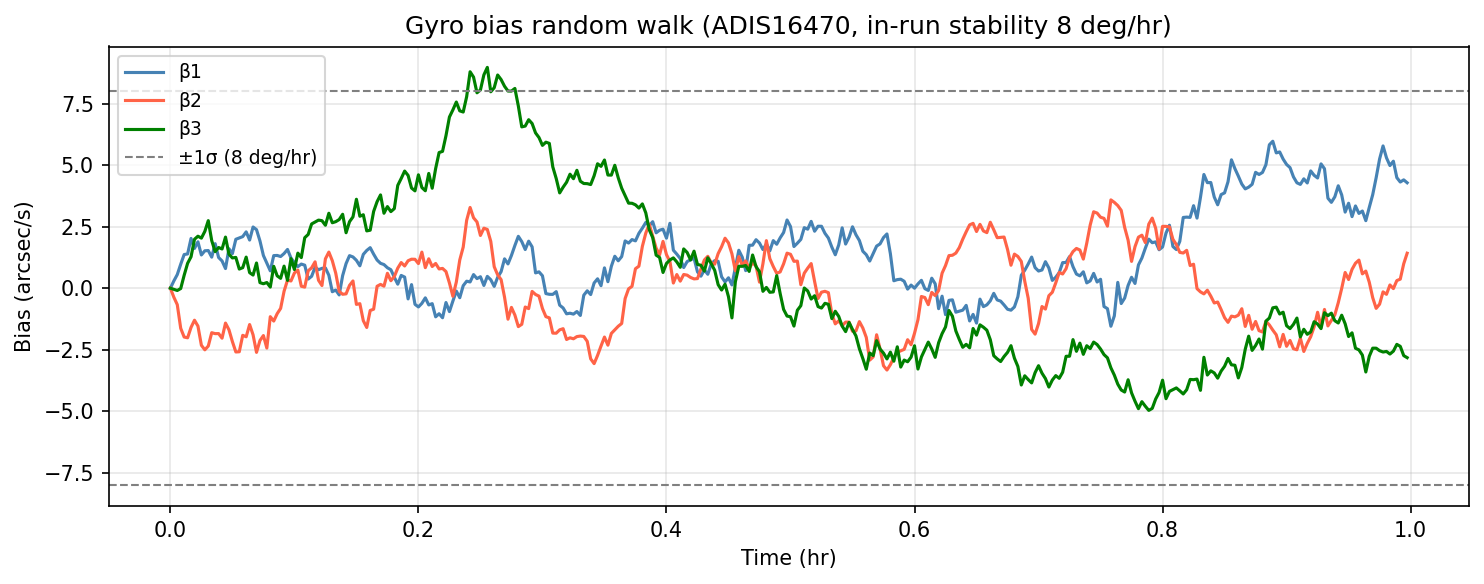
\includegraphics[width=0.82\linewidth]{figs/gyro_random_walk.png}
  \caption{Simulated ADIS16470 gyroscope bias random walk over one hour at 10 Hz.
    Dashed lines show the $\pm1\sigma$ (8 deg/hr) in-run bias stability envelope.}
  \label{fig:gyro_random_walk}
\end{figure}